
\noindent In the last lecture we introduced global conformal transformations/symmetries of some manifold $M$ that form a (symmetry) group $G$ which can be promoted to a symmetry group of some quanutm system, where the kinematics of the system are described by a Hilbert space $\mathcal{H}$. The quantum system is said to be globally conformally invariant if these is some unitary representation, operators $U$ that act on the Hilbert space,

\begin{equation}
U: \,\, G \rightarrow U(\mathcal{H}).
\end{equation}

\noindent Recall that in the generalized Minkowski space $\mathbb{R}^{p,q}$, the structure of the group of global conformal transformations $G$ consists of compositions of translations, dilations, rotations(boosts), and special conformal transformations (SCTs). \\

\noindent Here we now study the case where $d=2$, which will expand our notion of what a symmetry is and will allow us to define local, infinitesimal conformal transformations. \\

\noindent For example, a global conformal transformation, a $1-1$ differentiable map from $\mathbb{R}^2 \rightarrow \mathbb{R}^2$, may consist of a dilation and a rotation and look like

\begin{figure}[H]
	\centering
	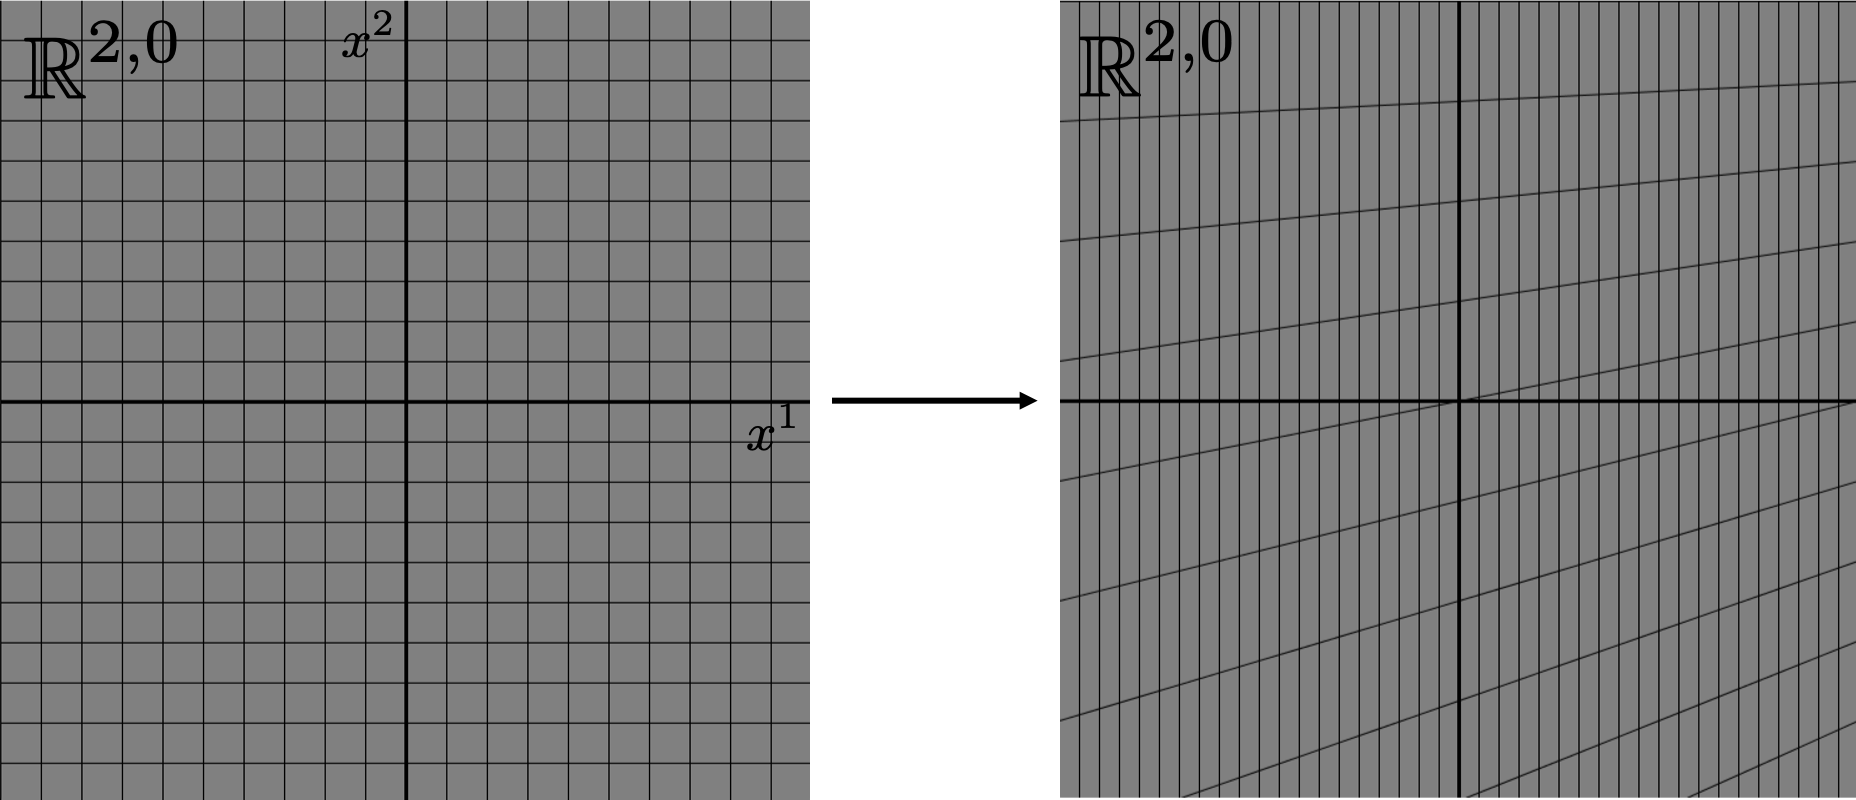
\includegraphics[width=4in]{images/global_conf_trans.png} 
\end{figure} 

\noindent For contrast, consider an infinitesimal conformal transformation $\text{id} + \epsilon X$, where $X=X(x)$ is a vector field, the derivative of a diffeomorphism, that acts on the two-dimensional Minkowski space as

\begin{figure}[H]
	\centering
	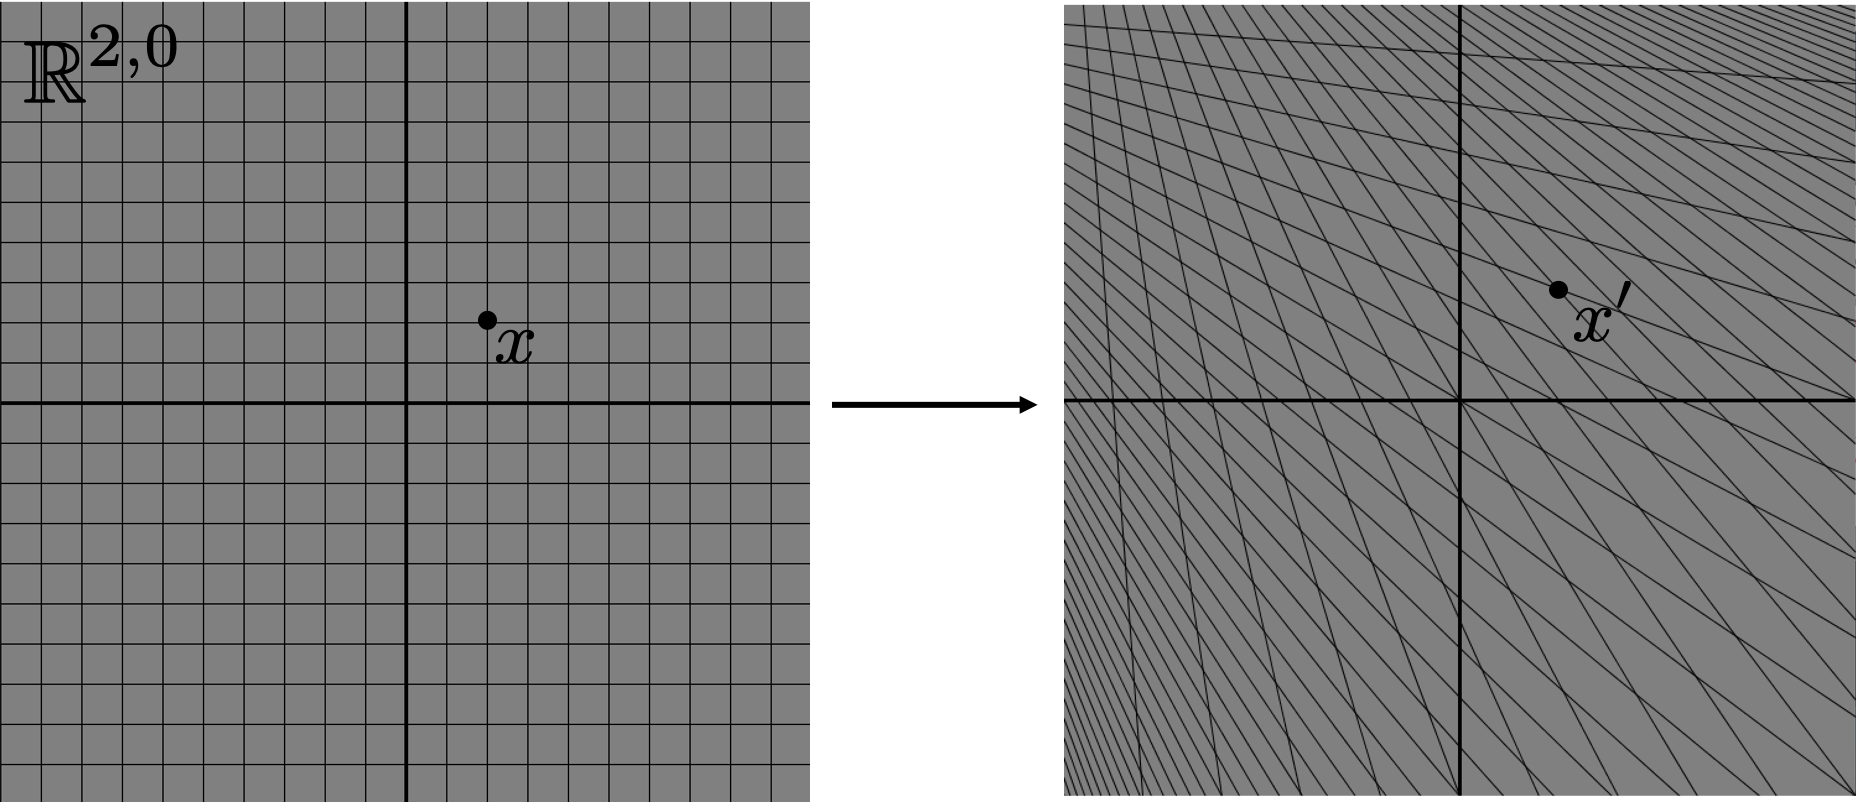
\includegraphics[width=4in]{images/inf_conf_trans.png} 
\end{figure} 

\noindent This transformation preserves all of the right angles in the untransformed Minkowski space, and the action is close to the identity, such that $|x-x'| \sim \mathcal{O}(\epsilon)$. The transformation $\text{id} + \epsilon X$ is conformal to first order in $\epsilon$, as is required by the definition of infinitesimal. \\

\noindent Although the vector field $X(x)$ is a generator of the infinitesimal conformal transformation, it does not necessarily define a global transformation via exponentiation, as it just may not be well defined globally.\\

\noindent To begin to make sense of this, consider in quantum mechanics, where we talk about quantum systems symmetric under a group $G$ with HIlbert space 

\begin{equation}
(\mathcal{H}, \,\, U: \, G \rightarrow U(\mathcal{H})).
\end{equation}

\noindent So, in quantum mechanics, we are reduced to finding these unitary representations of $G$. If $G$ is finite, it does not make sense to speak infinitesimally (e.g., one one-hundredth of a reflection). \\

\noindent We assume $G$ is a manifold, and then we may as well go as far to assume that $G$ is a Lie group with an associated Lie algebra $\mathfrak{g}$, which consists of vector fields that exponentiate to the Lie group. Then the quantum system is symmetric under the Lie algebra if you get a representation

\begin{equation}
(\mathcal{H}, \, \, \pi: \, \mathfrak{g} \rightarrow L(\mathcal{H}))
\end{equation}

\noindent Where $L(\mathcal{H})$ is the set of (bounded and unbounded) linear operators, and $\pi$ generates a unitary operator on the Hilbert space, such that $\pi(X)= e^{isX}$, $s\in \mathbb{R}$. \\

\noindent Note that for an infinite-dimensional group, (1) the operator $e^{isX}$ may not be continuous, and (2) the Lie algebra may not exponeniate to a Lie group, which we will encounter in conformal field theory. In other words, in contrast to when we used infinitesimal quanities to build global representations, we find that infinitesimal conformal transformations don't necessarily exponentiate to a group.\\

\noindent Therefore, in the infinitesimal case, we abandon looking for (full, continuous) unitary representations of the Lie group, and instead focus in on finding Hermitian representations that generate the Lie algebra. \\

\subsection*{Local algebra of infinitesimal conformal transformations}

\noindent Recall that for global conformal transformations, we have $z \rightarrow f(z)$, where $f$ is holomorphic with inverse $f^{-1}$. For infinitesimal $f$, this transformation, including the complex conjugate, becomes

\begin{equation}
z \rightarrow z + \epsilon (z) \text{ and } \bar{z} \rightarrow \bar{z} + \bar{\epsilon}(\bar{z})
\end{equation}

\noindent Where $\epsilon$ is a holomorphic function. A convenient choice of basis, which is infinite dimensional, is

\begin{equation}
\epsilon_n (z) = -\epsilon z^{n+1} \text{, where } n \in \mathbb{Z}.
\end{equation}

\noindent Given a diffeomorphism $[z \rightarrow z + \epsilon_n (z)] = e^{\epsilon \ell_n}$, the corresponding vector field tangent to every point in the manifold is defined by the operators

\begin{equation}
\ell_n \equiv - z^{n+1} \partial_z \text{ and } \bar{\ell}_n \equiv - \bar{z}^{n+1} \partial_{\bar{z}}.
\end{equation}

\noindent These differential operators form a basis, since they obey the commutation relations (\textbf{Exercise})

\begin{align}
[ \ell_m , \ell_n ] &= (m-n) \ell_{m+n} \\
[ \bar{\ell}_m, \bar{\ell}_n ] &= (m-n) \bar{\ell}_{m+n} \\
[\bar{\ell}_m , \ell_n ] &= 0.
\end{align}

\noindent They also as form a closed, infinite-dimensional Lie algebra $\forall m,n \in \mathbb{Z}$, called the Witt algebra $\text{WItt} = \mathcal{A} \oplus \bar{\mathcal{A}}$, where $\mathcal{A}$ is generated by $\{ \ell \}$, and $\bar{\mathcal{A}}$ is generated by $\{ \bar{\ell} \}$. Everything commutes in the basis, so the direct sum of the Witt algebra is justified. \\

\noindent The Witt algebra is generated infinitesimally, and could also be used to infinitiseimally generate a Lie group. This turns out to be true, but the Lie group is not the conformal group. \\

\noindent Which operators $\ell_n$ correspond to global transformations? \\

\noindent Consider a vector field 

\begin{equation}
v(z) = - \sum_{n=-\infty}^{\infty} v_n \ell_n = \sum_{n=-\infty}^{\infty} v_n z^{n+1} \partial_z.
\end{equation}

\noindent For this vector field to correspond to a global transformation, $v(z)$ must exponentiate to a holomorhpic map $f$, which is nonsingular in the limit as $z \rightarrow 0$. This places constraints on the coefficients of the vector field 

\begin{equation}
v_n = 0, \, n < -1.
\end{equation}

\noindent The inverse of the vector field must also exponentiate to a holomorphic map $f^{-1}$, which is nonsingular in the limit as $z \rightarrow \infty$ (e.g., exists on the Riemann sphere). This places the constraint on the coefficients of the vector field: 

\begin{equation}
v_n = 0, \, n>1.
\end{equation}

\noindent Note that if we demand holomorphism on the full complex plane without compactifying, the only allowed global transformations will be linear transformation (\textbf{Exercise}). By compactifying $\pm \infty$ as a point onto the Riemann sphere, we have more freedom in allowed global transformations. \\

\noindent With these constraints in place, we are left with three (six with complex conjugates) generators of infinitesimal global conformal transformations

\begin{equation}
\{ \ell_{-1}, \ell_0 , \ell_1 \} \cup \{ \bar{\ell}_{-1}, \bar{\ell}_0, \bar{\ell}_1 \}.
\end{equation}

\noindent The generators close to form a subalgebra under the commutator bracket $[,]$ defined above (\textbf{Exercise}), and generate thegroup of \textit{linear fractional (Moebius) transformations}, also known as the projective special linear group $\text{PSL}(2,\mathbb{C})$

\begin{equation}
z \rightarrow \frac{az + b}{c z + d}, \,\, ad-bc = 1.
\end{equation}

\noindent The set of global conformal transformations allowed in this basis are (\textbf{Exercise}), for $s \in \mathbb{R}$,

\begin{align}
&\text{Translation: } &e^{s \ell_{-1}} \equiv &\begin{pmatrix}1&-s \\ 0&1 \end{pmatrix} &\equiv z \rightarrow z - s \\
&\text{Dilation: } &e^{s (\ell_0 + \bar{\ell}_0)} \equiv &\begin{pmatrix}\lambda&0 \\ 0&\lambda^{-1} \end{pmatrix} &\equiv z \rightarrow e^{-s} \\
&\text{Rotation: } &e^{is (\bar{\ell}_0 - \ell_0)} \equiv &\begin{pmatrix}\text{exp}(i\frac{\theta}{2})&0 \\ 0&\text{exp}(-i\frac{\theta}{2}) \end{pmatrix} &\equiv z \rightarrow e^{is} \\
&\text{Special Conformal: } &e^{s \ell_1} \equiv &\begin{pmatrix}1&0 \\ c&1 \end{pmatrix} &\equiv z \rightarrow \frac{z}{1+c z}.
\end{align}

\noindent Note that for $\mathbb{R}^{d,0}$, $d>2$, the local transformations are also global! Also note that in one-dimensional spacetime, $(1,0)$ or $(0,1)$, conformal transformations are all monotonic increasing functions $\mathbb{R} \rightarrow \mathbb{R}$.

\subsection*{$d=2$ Minkowski space, $\mathbb{R}^{1,1}$}

\noindent The conformal group  of $\mathbb{R}^{1,1}$ is \textit{special}. \\

\noindent \textbf{Theorem:} \\

\noindent A smooth map $\varphi = (u,v) : \, M \rightarrow \mathbb{R}^{1,1}$ from a connected subset of $M \subset \mathbb{R}^{1,1}$ is conformal (pulls back metric to a scalar multiple of the diagonal metric), iff $u_x^2 > v_x^2$ and $u_x = v_y,\, u_y = v_x$ or $u_x = -v_y,\, u_y = -v_x$. \\

\begin{figure}[H]
	\centering
	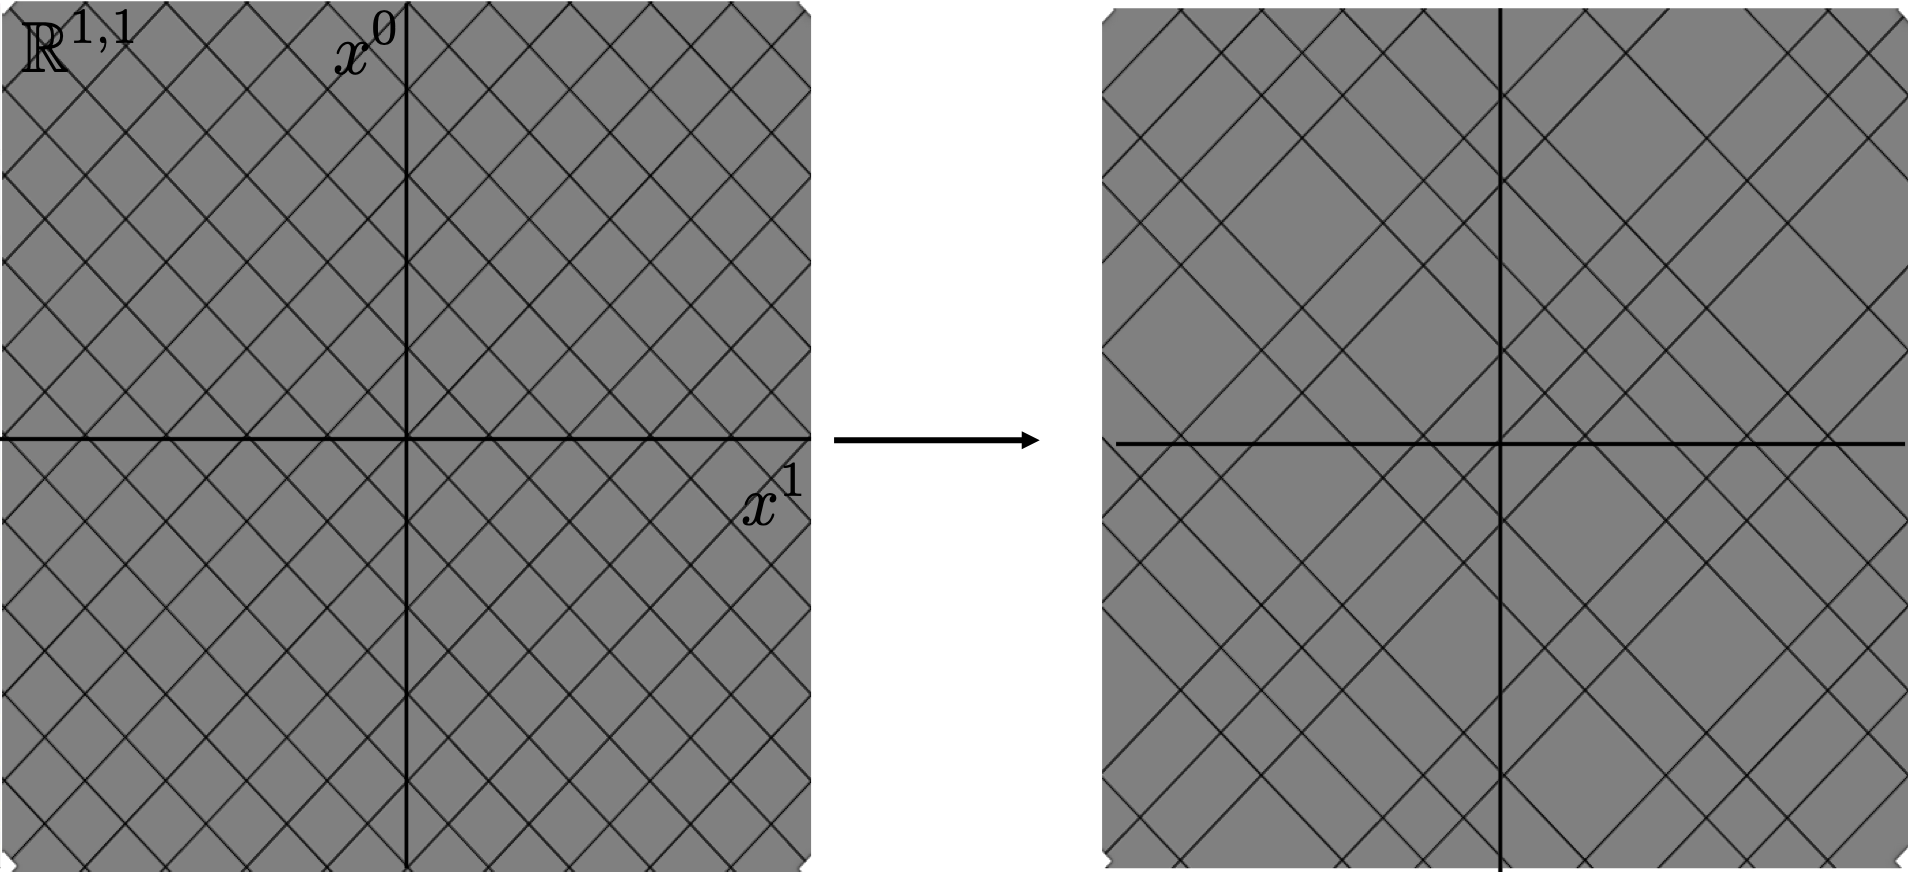
\includegraphics[width=4in]{images/conf_trans_lightcone.png} 
\end{figure} 

\noindent \textbf{Theorem:} \\

\noindent Consider an infinitely differentiable function on the real line $f \in C^\infty (\mathbb{R})$, and let $f_\pm \in C^\infty (\mathbb{R}^2, \mathbb{R})$, the infinitely differentiable functions from the real line to the real plane, be defined by $f_\pm (x,y) = f(x \pm y)$. Then the map 

\begin{align}
\Phi: \, C^\infty (\mathbb{R}) \times C^\infty (\mathbb{R}) &\rightarrow C^\infty (\mathbb{R}^2, \mathbb{R}^2) \\
(f,g) &\rightarrow \frac{1}{2} (f_+ + g_-, f_+ - g_- )
\end{align}

\noindent Has the following properties

\begin{itemize}
\item image($\Phi$) $= \{ (u,v): \, u_x = v_y, \, u_y, v_x \}$
\item $\Phi(f,g)$ is conformal iff $f'>0$ and $g' >0$ or $f'<0$ and $g'<0$
\item $\Phi$ is bijective iff $f$ and $g$ are bijective
\item $\Phi(f \circ h, g \circ k) = \Phi(f,g) \circ \Phi (h,k), \forall f,g,h,k \in C^\infty(\mathbb{R}) \equiv \Phi$ is a homomorphism.
\end{itemize}

\noindent The group of orientation-preserving transformations of $M=\mathbb{R}^{1,1}$ is isomorphic to 

\begin{equation}
(\text{Diff}_+ (\mathbb{R}) \times \text{Diff}_+ (\mathbb{R})) \cup (\text{Diff}_- (\mathbb{R}) \times \text{Diff}_- (\mathbb{R}))
\end{equation}

\noindent Which consists of the infinitely-differentiable orientation-preserving maps of $\mathbb{R}$, diffeomorphisms of $\mathbb{R}$. \\

\noindent It is convenient to compactify $\mathbb{R}^{1,1} \rightarrow S^{1,1} \subset \mathbb{R}^{2,0} \times \mathbb{R}^{0,2}$. Then the group of orientation-preserving transformations of $M=S^{1,1}$ is isomorphic to 

\begin{equation}
\text{Conf} (\mathbb{R}^{1,1}) \equiv (\text{Diff}_+ (S^1) \times \text{Diff}_+ (S^1)) \cup (\text{Diff}_- (S^1) \times \text{Diff}_- (S^1)).
\end{equation}

\noindent This is the definition of the conformal group of Minkowski space. Typically, we throw away the second part of the union, the $''-''$ reversing part, since it is the same as preserving with $z \rightarrow -z$, and focus on the infinite-dimensional subgroup $\text{Diff}_+ (S^1)$, which we call the \textit{chiral half} of the conformal group. This is admissable, since the symmetries of a quantum system can be understood by the symmetries of $\text{Diff}_+ (S^1)$, and the rest is easily gotten by tensor products to include the other light-cone axes. \\

\noindent In the next lecture, we will focus on which quantum systems are invariant under this infinite-dimensional group $\text{Diff}_+ (S^1)$ by going to the Lie algebra, which turns out to be isomorphic to the Witt algebra, in the Euclidean case. The unitary representations, gotten via infinitesimal generators, of $\text{Diff}_+ (S^1)$ will not be bounded below and are unstable. Therefore, \textit{projective} unitary representaitons will be required, and are classified by the \textit{central charge}.